\section*{Лекція 12: Помилки та виключення}
 
 \subsection{Вступ в обробку виключень} 
\begin{frame}
\frametitle{Види виключень}
Виключення бувають:
\begin{itemize}
  \item в процесі виконання програми (можна оброблювати);
  \item в процесі компіляції програми (треба правильно писати програму).
\end{itemize}
\begin{figure}
  \begin{center}
    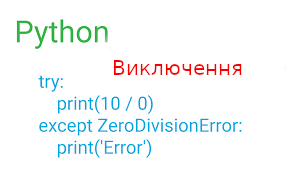
\includegraphics[width=0.4\textwidth,height=0.4\textheight]{pictures/exceptions.png}
  \caption{Виключення}
\label{function}
  \end{center}
\end{figure}


\end{frame}

\begin{frame}
\frametitle{<<Відловлювання>> виключень}

\texttt{try:}

\texttt{~~~~operations\_1}

\texttt{except error\_1:}

\texttt{~~~~operations\_2}

\texttt{except error\_2:}

\texttt{~~~~operations\_3}

\vspace{0.5cm}
При <<відловлюванні>> виключень враховується ієрархія класів виключень.
\end{frame}

\begin{frame}
\frametitle{Класи виключень}
\begin{figure}
\begin{center}
 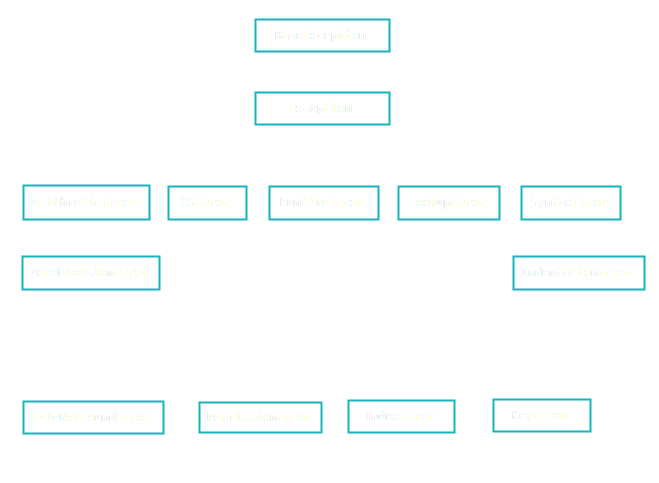
\includegraphics[width=0.6\textwidth]{pictures/exception.png}
\caption{Виключення}
\label{exception} 
\end{center}
\end{figure}

\end{frame}

\begin{frame}
\frametitle{Конструкція try-except-else-finally}
\texttt{try:}

\texttt{~~~~operations\_1}

\texttt{except error\_1 as val:}

\texttt{~~~~operations\_2}

\texttt{else:}

\texttt{~~~~operations\_3}

\texttt{finally:}

\texttt{~~~~operations\_4}

\texttt{val} - екземпляр класу виключення. \texttt{operations\_3} - виконуються при штатному завершенні \texttt{operations\_1}. \texttt{operations\_4} - виконуються завжди (до \texttt{return}).
\end{frame}

\begin{frame}
\frametitle{Виключення та стек виклику функцій}
При виникненні виключень всередині функцій вони розповсюджуються по стеку виклику функцій.

Оброблювати виключення можна на будь-якому рівні стеку.

\begin{figure}
  \begin{center}
    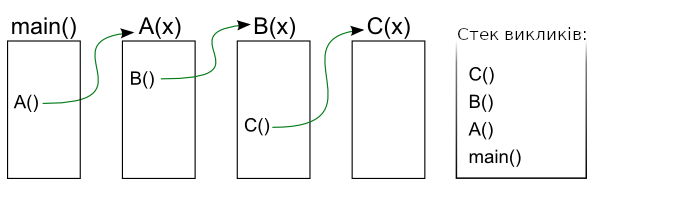
\includegraphics[width=0.8\textwidth,height=0.4\textheight]{pictures/stack.png}
  \caption{Стек виклику функцій}
\label{function}
  \end{center}
\end{figure}
\end{frame}

\subsection{Генерація виключень} 
\begin{frame}
\frametitle{Генерація виключень}
\begin{figure}
  \begin{center}
    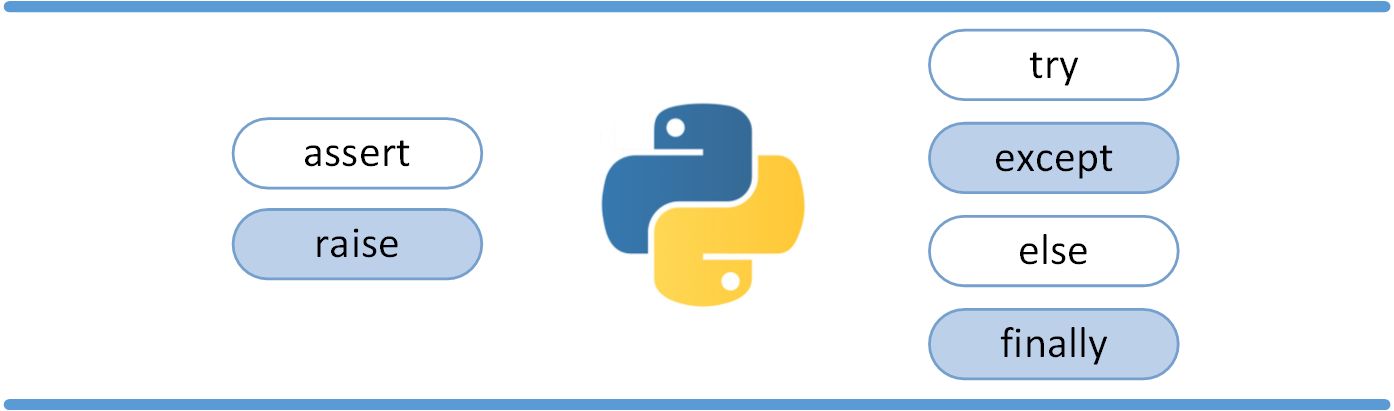
\includegraphics[width=0.4\textwidth,height=0.2\textheight]{pictures/assert-raise.png}
  \caption{Генерація виключень}
\label{function}
  \end{center}
\end{figure}

Трапляються ситуації, коли формально помилки немає, але змінна набуває непотрібного значення. Тоді можна згенерувати виключення за допомогою функцій \texttt{assert} або \texttt{raise}.

\end{frame}

\begin{frame}
\frametitle{Функція raise}
\texttt{try:}
    
\texttt{~~~~value = int(input())}

\texttt{~~~~if value \% 2 != 0:}

\texttt{~~~~~~~~raise ValueError('Value must be even!')}

\texttt{~~~~print('Congratulations! Value is even!')}

\texttt{except Exception as e:}

\texttt{~~~~print(f'{e.\_\_class\_\_}: {e}')}

Прийнято використовувати клас \texttt{Exception}. Можна створювати власні класи, що успадковуються від класу \texttt{Exception}, та <<ловити>> їх за допомогою \texttt{try/except}.
\end{frame}


\begin{frame}
\frametitle{Функція assert}

\texttt{try:}
    
\texttt{~~~~value = int(input())}

\texttt{~~~~assert value \% 2 == 0, 'Value must be even!'}

\texttt{~~~~print('Congratulations! Value is even!')}

\texttt{except Exception as e:}

\texttt{~~~~print(f'{e.\_\_class\_\_}: {e}')}

\begin{enumerate}
  \item assert не вимагає окремого блоку if — перевірка відбувається в один рядок;
  \item для assert клас виключення — AssertionError.

\end{enumerate}
\end{frame}
